\documentclass[11pt]{article}
\usepackage{geometry,marginnote} % Pour passer au format A4
\geometry{hmargin=1cm, vmargin=1cm} % 

% Page et encodage
\usepackage[T1]{fontenc} % Use 8-bit encoding that has 256 glyphs
\usepackage[english,french]{babel} % Français et anglais
\usepackage[utf8]{inputenc} 

\usepackage{lmodern,numprint}
\setlength\parindent{0pt}

% Graphiques
\usepackage{graphicx,float,grffile,units}
\usepackage{tikz,pst-eucl,pst-plot,pstricks,pst-node,pstricks-add,pst-fun,pgfplots} 

% Maths et divers
\usepackage{amsmath,amsfonts,amssymb,amsthm,verbatim}
\usepackage{multicol,enumitem,url,eurosym,gensymb,tabularx}

\DeclareUnicodeCharacter{20AC}{\euro}



% Sections
\usepackage{sectsty} % Allows customizing section commands
\allsectionsfont{\centering \normalfont\scshape}

% Tête et pied de page
\usepackage{fancyhdr} \pagestyle{fancyplain} \fancyhead{} \fancyfoot{}

\renewcommand{\headrulewidth}{0pt} % Remove header underlines
\renewcommand{\footrulewidth}{0pt} % Remove footer underlines

\newcommand{\horrule}[1]{\rule{\linewidth}{#1}} % Create horizontal rule command with 1 argument of height

\newcommand{\Pointilles}[1][3]{%
  \multido{}{#1}{\makebox[\linewidth]{\dotfill}\\[\parskip]
}}

\newtheorem{Definition}{Définition}

\usepackage{siunitx}
\sisetup{
    detect-all,
    output-decimal-marker={,},
    group-minimum-digits = 3,
    group-separator={~},
    number-unit-separator={~},
    inter-unit-product={~}
}

\setlength{\columnseprule}{1pt}

\begin{document}

\textbf{Nom, Prénom :} \hspace{8cm} \textbf{Classe :} \hspace{3cm} \textbf{Date :}\\
\vspace{-0.8cm}
\begin{center}
  \textit{Je n'aime pas le travail, nul ne l'aime ; mais j'aime ce qui est dans le travail l'occasion de se découvrir soi-même.}  - \textbf{Joseph Conrad}
\end{center}
\vspace{-0.8cm}

\subsection*{Définitions}
  \begin{enumerate}
    \item[1.] Fraction partage: \dotfill \\
    \Pointilles[1]
  \end{enumerate}

  \vspace{-1cm}

\subsection*{Exercice 1 - Bande unité}

Plier et coller une bande unité en la partageant en $\dfrac{4}{6}$.

\vspace{2cm}

\subsection*{Exercice 2 - Fractions unités}

Écrire la fraction correspondante au partage de l'unité de chacune des bandes. 

\begin{figure}[H]
    \centering
    \includegraphics[width=0.6\linewidth]{6x1-fraction-partage/6x1-exo1a.pdf}
  \end{figure}


\subsection*{Exercice 3 - Calculer}

\begin{enumerate}
    \item[a.] $\dfrac{1}{4} + \dfrac{1}{4} = $ \dotfill
    \item[b.] $\dfrac{2}{51} + \dfrac{10}{51} + \dfrac{3}{51} = $ \dotfill
    \item[c.] $2 \times \dfrac{1}{6} = $ \dotfill
    \item[d.] $\dfrac{856}{856}$ \dotfill
    \item[e.] un quart plus un quart égal \dotfill
    \item[f.] cinq douzième moins deux douzième égal \dotfill
 \end{enumerate}


\subsection*{Sudoku 4x4}

\begin{figure}[H]
  \centering
  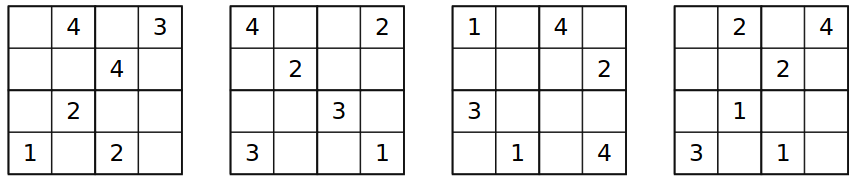
\includegraphics[width=0.8\linewidth]{6x1-fraction-partage/sudoku-4a.png}
\end{figure}

\newpage

\textbf{Nom, Prénom :} \hspace{8cm} \textbf{Classe :} \hspace{3cm} \textbf{Date :}\\
\vspace{-0.8cm}
\begin{center}
  \textit{Je n'aime pas le travail, nul ne l'aime ; mais j'aime ce qui est dans le travail l'occasion de se découvrir soi-même.}  - \textbf{Joseph Conrad}
\end{center}
\vspace{-0.8cm}

\subsection*{Définitions}
  \begin{enumerate}
    \item[1.] Fraction partage: \dotfill \\
    \Pointilles[1]
  \end{enumerate}

  \vspace{-1cm}

\subsection*{Exercice 1 - Bande unité}

Plier et coller une bande unité en la partageant en $\dfrac{4}{6}$.

\vspace{2cm}

\subsection*{Exercice 2 - Fractions unités}

Écrire la fraction correspondante au partage de l'unité de chacune des bandes. 

\begin{figure}[H]
    \centering
    \includegraphics[width=0.6\linewidth]{6x1-fraction-partage/6x1-exo1b.pdf}
  \end{figure}


\subsection*{Exercice 3 - Calculer}

\begin{enumerate}
    \item[a.] $\dfrac{1}{3} + \dfrac{1}{3} = $ \dotfill
    \item[b.] $\dfrac{4}{37} + \dfrac{10}{37} + \dfrac{2}{37} = $ \dotfill
    \item[c.] $2 \times \dfrac{1}{8} = $ \dotfill
    \item[d.] $\dfrac{759}{759}$ \dotfill
    \item[e.] un tiers plus un tiers égal \dotfill
    \item[f.] sept quinzième moins deux quinzième égal \dotfill
 \end{enumerate}


\subsection*{Sudoku 4x4}

\begin{figure}[H]
  \centering
  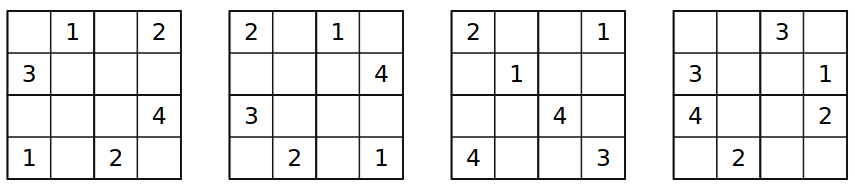
\includegraphics[width=0.8\linewidth]{6x1-fraction-partage/sudoku-4b.png}
\end{figure}

\end{document}